% Options for packages loaded elsewhere
\PassOptionsToPackage{unicode}{hyperref}
\PassOptionsToPackage{hyphens}{url}
%
\documentclass[
]{book}
\usepackage{lmodern}
\usepackage{amssymb,amsmath}
\usepackage{ifxetex,ifluatex}
\ifnum 0\ifxetex 1\fi\ifluatex 1\fi=0 % if pdftex
  \usepackage[T1]{fontenc}
  \usepackage[utf8]{inputenc}
  \usepackage{textcomp} % provide euro and other symbols
\else % if luatex or xetex
  \usepackage{unicode-math}
  \defaultfontfeatures{Scale=MatchLowercase}
  \defaultfontfeatures[\rmfamily]{Ligatures=TeX,Scale=1}
\fi
% Use upquote if available, for straight quotes in verbatim environments
\IfFileExists{upquote.sty}{\usepackage{upquote}}{}
\IfFileExists{microtype.sty}{% use microtype if available
  \usepackage[]{microtype}
  \UseMicrotypeSet[protrusion]{basicmath} % disable protrusion for tt fonts
}{}
\makeatletter
\@ifundefined{KOMAClassName}{% if non-KOMA class
  \IfFileExists{parskip.sty}{%
    \usepackage{parskip}
  }{% else
    \setlength{\parindent}{0pt}
    \setlength{\parskip}{6pt plus 2pt minus 1pt}}
}{% if KOMA class
  \KOMAoptions{parskip=half}}
\makeatother
\usepackage{xcolor}
\IfFileExists{xurl.sty}{\usepackage{xurl}}{} % add URL line breaks if available
\IfFileExists{bookmark.sty}{\usepackage{bookmark}}{\usepackage{hyperref}}
\hypersetup{
  pdftitle={GEO Data Tutorial},
  pdfauthor={Kyle Roell},
  hidelinks,
  pdfcreator={LaTeX via pandoc}}
\urlstyle{same} % disable monospaced font for URLs
\usepackage{color}
\usepackage{fancyvrb}
\newcommand{\VerbBar}{|}
\newcommand{\VERB}{\Verb[commandchars=\\\{\}]}
\DefineVerbatimEnvironment{Highlighting}{Verbatim}{commandchars=\\\{\}}
% Add ',fontsize=\small' for more characters per line
\usepackage{framed}
\definecolor{shadecolor}{RGB}{248,248,248}
\newenvironment{Shaded}{\begin{snugshade}}{\end{snugshade}}
\newcommand{\AlertTok}[1]{\textcolor[rgb]{0.94,0.16,0.16}{#1}}
\newcommand{\AnnotationTok}[1]{\textcolor[rgb]{0.56,0.35,0.01}{\textbf{\textit{#1}}}}
\newcommand{\AttributeTok}[1]{\textcolor[rgb]{0.77,0.63,0.00}{#1}}
\newcommand{\BaseNTok}[1]{\textcolor[rgb]{0.00,0.00,0.81}{#1}}
\newcommand{\BuiltInTok}[1]{#1}
\newcommand{\CharTok}[1]{\textcolor[rgb]{0.31,0.60,0.02}{#1}}
\newcommand{\CommentTok}[1]{\textcolor[rgb]{0.56,0.35,0.01}{\textit{#1}}}
\newcommand{\CommentVarTok}[1]{\textcolor[rgb]{0.56,0.35,0.01}{\textbf{\textit{#1}}}}
\newcommand{\ConstantTok}[1]{\textcolor[rgb]{0.00,0.00,0.00}{#1}}
\newcommand{\ControlFlowTok}[1]{\textcolor[rgb]{0.13,0.29,0.53}{\textbf{#1}}}
\newcommand{\DataTypeTok}[1]{\textcolor[rgb]{0.13,0.29,0.53}{#1}}
\newcommand{\DecValTok}[1]{\textcolor[rgb]{0.00,0.00,0.81}{#1}}
\newcommand{\DocumentationTok}[1]{\textcolor[rgb]{0.56,0.35,0.01}{\textbf{\textit{#1}}}}
\newcommand{\ErrorTok}[1]{\textcolor[rgb]{0.64,0.00,0.00}{\textbf{#1}}}
\newcommand{\ExtensionTok}[1]{#1}
\newcommand{\FloatTok}[1]{\textcolor[rgb]{0.00,0.00,0.81}{#1}}
\newcommand{\FunctionTok}[1]{\textcolor[rgb]{0.00,0.00,0.00}{#1}}
\newcommand{\ImportTok}[1]{#1}
\newcommand{\InformationTok}[1]{\textcolor[rgb]{0.56,0.35,0.01}{\textbf{\textit{#1}}}}
\newcommand{\KeywordTok}[1]{\textcolor[rgb]{0.13,0.29,0.53}{\textbf{#1}}}
\newcommand{\NormalTok}[1]{#1}
\newcommand{\OperatorTok}[1]{\textcolor[rgb]{0.81,0.36,0.00}{\textbf{#1}}}
\newcommand{\OtherTok}[1]{\textcolor[rgb]{0.56,0.35,0.01}{#1}}
\newcommand{\PreprocessorTok}[1]{\textcolor[rgb]{0.56,0.35,0.01}{\textit{#1}}}
\newcommand{\RegionMarkerTok}[1]{#1}
\newcommand{\SpecialCharTok}[1]{\textcolor[rgb]{0.00,0.00,0.00}{#1}}
\newcommand{\SpecialStringTok}[1]{\textcolor[rgb]{0.31,0.60,0.02}{#1}}
\newcommand{\StringTok}[1]{\textcolor[rgb]{0.31,0.60,0.02}{#1}}
\newcommand{\VariableTok}[1]{\textcolor[rgb]{0.00,0.00,0.00}{#1}}
\newcommand{\VerbatimStringTok}[1]{\textcolor[rgb]{0.31,0.60,0.02}{#1}}
\newcommand{\WarningTok}[1]{\textcolor[rgb]{0.56,0.35,0.01}{\textbf{\textit{#1}}}}
\usepackage{longtable,booktabs}
% Correct order of tables after \paragraph or \subparagraph
\usepackage{etoolbox}
\makeatletter
\patchcmd\longtable{\par}{\if@noskipsec\mbox{}\fi\par}{}{}
\makeatother
% Allow footnotes in longtable head/foot
\IfFileExists{footnotehyper.sty}{\usepackage{footnotehyper}}{\usepackage{footnote}}
\makesavenoteenv{longtable}
\usepackage{graphicx,grffile}
\makeatletter
\def\maxwidth{\ifdim\Gin@nat@width>\linewidth\linewidth\else\Gin@nat@width\fi}
\def\maxheight{\ifdim\Gin@nat@height>\textheight\textheight\else\Gin@nat@height\fi}
\makeatother
% Scale images if necessary, so that they will not overflow the page
% margins by default, and it is still possible to overwrite the defaults
% using explicit options in \includegraphics[width, height, ...]{}
\setkeys{Gin}{width=\maxwidth,height=\maxheight,keepaspectratio}
% Set default figure placement to htbp
\makeatletter
\def\fps@figure{htbp}
\makeatother
\setlength{\emergencystretch}{3em} % prevent overfull lines
\providecommand{\tightlist}{%
  \setlength{\itemsep}{0pt}\setlength{\parskip}{0pt}}
\setcounter{secnumdepth}{5}
\usepackage{booktabs}
\usepackage[]{natbib}
\bibliographystyle{plainnat}

\title{GEO Data Tutorial}
\author{Kyle Roell}
\date{2021-06-03}

\begin{document}
\maketitle

{
\setcounter{tocdepth}{1}
\tableofcontents
}
\hypertarget{gene-expression-omnibus-geo}{%
\chapter{Gene Expression Omnibus (GEO)}\label{gene-expression-omnibus-geo}}

GEO is a public functional genomics data repository supporting MIAME-compliant data submissions. Array- and sequence-based data are accepted. Tools are provided to help users query and download experiments and curated gene expression profiles.

We will be using GEO to access and download data to perform various statistical and graphic procedures.

Data in this tutorial will be downloaded from \href{https://www.ncbi.nlm.nih.gov/geo/query/acc.cgi?acc=GSE42394}{GSE42394}.

The entire RMarkdown code can be found on our \href{https://github.com/kyleroell/test}{UNC-SRP Github site}.


\includegraphics{~/Downloads/UNC-SRP Graphic ID FOR SCREEN_RGB.jpg}

\hypertarget{geoquery}{%
\chapter{Loading and Manipulating GEO Data}\label{geoquery}}

The \href{https://www.bioconductor.org/packages/release/bioc/html/GEOquery.html}{GEOquery package} allows for easy reading in and downloading data from GEO. This will parse the data for you and store it into an R object that you can reference and manipulate for data analysis.

You can both read in data from a file that has manually been downloaded from GEO or let GEOquery download the data for you. Here, we will show how to simply read in a file that we have already downloaded from GEO. All we need to download is the same file that we manipulated in Method 1 above!

\begin{Shaded}
\begin{Highlighting}[]
\CommentTok{#First install GEOquery}
\ControlFlowTok{if}\NormalTok{ (}\OperatorTok{!}\KeywordTok{requireNamespace}\NormalTok{(}\StringTok{"BiocManager"}\NormalTok{, }\DataTypeTok{quietly =} \OtherTok{TRUE}\NormalTok{))}
    \KeywordTok{install.packages}\NormalTok{(}\StringTok{"BiocManager"}\NormalTok{);}

\NormalTok{BiocManager}\OperatorTok{::}\KeywordTok{install}\NormalTok{(}\StringTok{"GEOquery"}\NormalTok{);}

\CommentTok{#load the package}
\KeywordTok{library}\NormalTok{(GEOquery);}

\CommentTok{#Now we can use the getGEO function to load data from our series matrix}
\NormalTok{geo.getGEO.data =}\StringTok{ }\KeywordTok{getGEO}\NormalTok{(}\DataTypeTok{filename=}\StringTok{'~/Downloads/GSE42394_series_matrix.txt'}\NormalTok{);}

\CommentTok{#We can get a dataset with the sample information using the pData() function}
\NormalTok{sampleInfo <-}\StringTok{ }\KeywordTok{pData}\NormalTok{(geo.getGEO.data);}

\CommentTok{#Let's look at some of our sample information dataset columns}
\NormalTok{knitr}\OperatorTok{::}\KeywordTok{kable}\NormalTok{(}
  \KeywordTok{head}\NormalTok{(sampleInfo[,}\KeywordTok{c}\NormalTok{(}\StringTok{"geo_accession"}\NormalTok{, }\StringTok{"cell type:ch1"}\NormalTok{, }\StringTok{"time:ch1"}\NormalTok{,}
                     \StringTok{"treatment:ch1"}\NormalTok{)]), }\DataTypeTok{caption =} \StringTok{'Sample information column names'}\NormalTok{,}
  \DataTypeTok{booktabs =} \OtherTok{TRUE}
\NormalTok{)}
\end{Highlighting}
\end{Shaded}

\begin{table}

\caption{\label{tab:load2}Sample information column names}
\centering
\begin{tabular}[t]{lllll}
\toprule
  & geo\_accession & cell type:ch1 & time:ch1 & treatment:ch1\\
\midrule
GSM1150937 & GSM1150937 & Nasal epithelial cells & 7 day & unexposed\\
GSM1150938 & GSM1150938 & Nasal epithelial cells & 7 day & unexposed\\
GSM1150939 & GSM1150939 & Nasal epithelial cells & 7 day & unexposed\\
GSM1150940 & GSM1150940 & Nasal epithelial cells & 7 day & 2 ppm formaldehyde\\
GSM1150941 & GSM1150941 & Nasal epithelial cells & 7 day & 2 ppm formaldehyde\\
\addlinespace
GSM1150942 & GSM1150942 & Nasal epithelial cells & 7 day & 2 ppm formaldehyde\\
\bottomrule
\end{tabular}
\end{table}

Now, we can use this to just define the samples we want to analyze.

We only want cell type = Nasal epithelial cells and time = 7 day. To do this, we can use our sampleInfo dataset and the variables ``cell type:ch1'' and ``time:ch1''. We will also define treated and untreated using the variable ``treatment:ch1''.

\begin{Shaded}
\begin{Highlighting}[]
\CommentTok{#Define keep variable that will store rows we want to keep}
\NormalTok{keep =}\StringTok{ }\KeywordTok{rownames}\NormalTok{(sampleInfo[}\KeywordTok{which}\NormalTok{(sampleInfo}\OperatorTok{$}\StringTok{`}\DataTypeTok{cell type:ch1}\StringTok{`}\OperatorTok{==}\StringTok{"Nasal epithelial cells"} 
                                 \OperatorTok{&}\StringTok{ }\NormalTok{sampleInfo}\OperatorTok{$}\StringTok{`}\DataTypeTok{time:ch1}\StringTok{`}\OperatorTok{==}\StringTok{"7 day"}\NormalTok{),]);}

\CommentTok{#first let's just subset sample info for just those samples we defined in keep variable}
\NormalTok{sampleInfo =}\StringTok{ }\NormalTok{sampleInfo[keep,];}

\CommentTok{#get the treated and untreated sample ids }
\CommentTok{#(which are in the variable geo_accession)}
\NormalTok{treated  =}\StringTok{ }\NormalTok{sampleInfo[}\KeywordTok{which}\NormalTok{(sampleInfo}\OperatorTok{$}\StringTok{`}\DataTypeTok{treatment:ch1}\StringTok{`}\OperatorTok{==}\StringTok{"2 ppm formaldehyde"}\NormalTok{), }
                      \StringTok{"geo_accession"}\NormalTok{];}
\NormalTok{untreated  =}\StringTok{ }\NormalTok{sampleInfo[}\KeywordTok{which}\NormalTok{(sampleInfo}\OperatorTok{$}\StringTok{`}\DataTypeTok{treatment:ch1}\StringTok{`}\OperatorTok{==}\StringTok{"unexposed"}\NormalTok{), }
                        \StringTok{"geo_accession"}\NormalTok{];}
\end{Highlighting}
\end{Shaded}

We now have a list of the samples we want to keep, stored in our variable ``keep''. The next step is to actually get the data we want to use in our analyses. The GEOquery function exprs() allows us to easily get this data.

\begin{Shaded}
\begin{Highlighting}[]
\CommentTok{#We can get the actual data using the exprs() function}
\CommentTok{#and we only want to keep those we previously defined}
\NormalTok{ge.data =}\StringTok{ }\KeywordTok{exprs}\NormalTok{(geo.getGEO.data[,keep]);}

\CommentTok{#Let's look at our sample information dataset}
\NormalTok{knitr}\OperatorTok{::}\KeywordTok{kable}\NormalTok{(}
\NormalTok{  ge.data[}\DecValTok{1}\OperatorTok{:}\DecValTok{5}\NormalTok{,}\DecValTok{1}\OperatorTok{:}\DecValTok{5}\NormalTok{], }\DataTypeTok{caption =} \StringTok{'Gene expression data'}\NormalTok{,}
  \DataTypeTok{booktabs =} \OtherTok{TRUE}
\NormalTok{)}
\end{Highlighting}
\end{Shaded}

\begin{table}

\caption{\label{tab:load2b}Gene expression data}
\centering
\begin{tabular}[t]{lrrrrr}
\toprule
  & GSM1150937 & GSM1150938 & GSM1150939 & GSM1150940 & GSM1150941\\
\midrule
10700001 & 5786.60 & 5830.08 & 5637.34 & 5313.33 & 5557.04\\
10700002 & 192.92 & 206.86 & 220.83 & 183.12 & 177.16\\
10700003 & 1820.98 & 1795.79 & 1735.70 & 1578.02 & 1681.58\\
10700004 & 66.95 & 65.61 & 64.41 & 60.19 & 60.41\\
10700005 & 770.07 & 753.41 & 731.20 & 684.53 & 657.25\\
\bottomrule
\end{tabular}
\end{table}

\hypertarget{statistical-procedures}{%
\chapter{Statistical Procedures}\label{statistical-procedures}}

\hypertarget{t-test}{%
\section{T-Test}\label{t-test}}

One of the most basic statistical procedures we can perform on this dataset is a set of t-tests to test for differences between the two treatment groups (exposed and unexposed) across each of the genes. One way to do this is to use a loop and test each gene individually, saving the p-value from the t-test into a separate dataframe. Another solution is to use the build in ``apply'' function. This function will return results obtained by applying a specified function (the ``t.test'' function) to the margins of our dataset.

\begin{Shaded}
\begin{Highlighting}[]
\CommentTok{#Use ge.data dataset}
\CommentTok{#use the t.test function comparing treated and untreated samples}
\CommentTok{#1 specifies to apply the function to rows}
\NormalTok{pValues <-}\StringTok{ }\KeywordTok{apply}\NormalTok{(ge.data, }\DecValTok{1}\NormalTok{, }\ControlFlowTok{function}\NormalTok{(x) }\KeywordTok{t.test}\NormalTok{(x[treated],x[untreated])}\OperatorTok{$}\NormalTok{p.value);}

\CommentTok{#We can look at a histogram of the pvalues to see distribution}
\KeywordTok{hist}\NormalTok{(pValues);}
\end{Highlighting}
\end{Shaded}

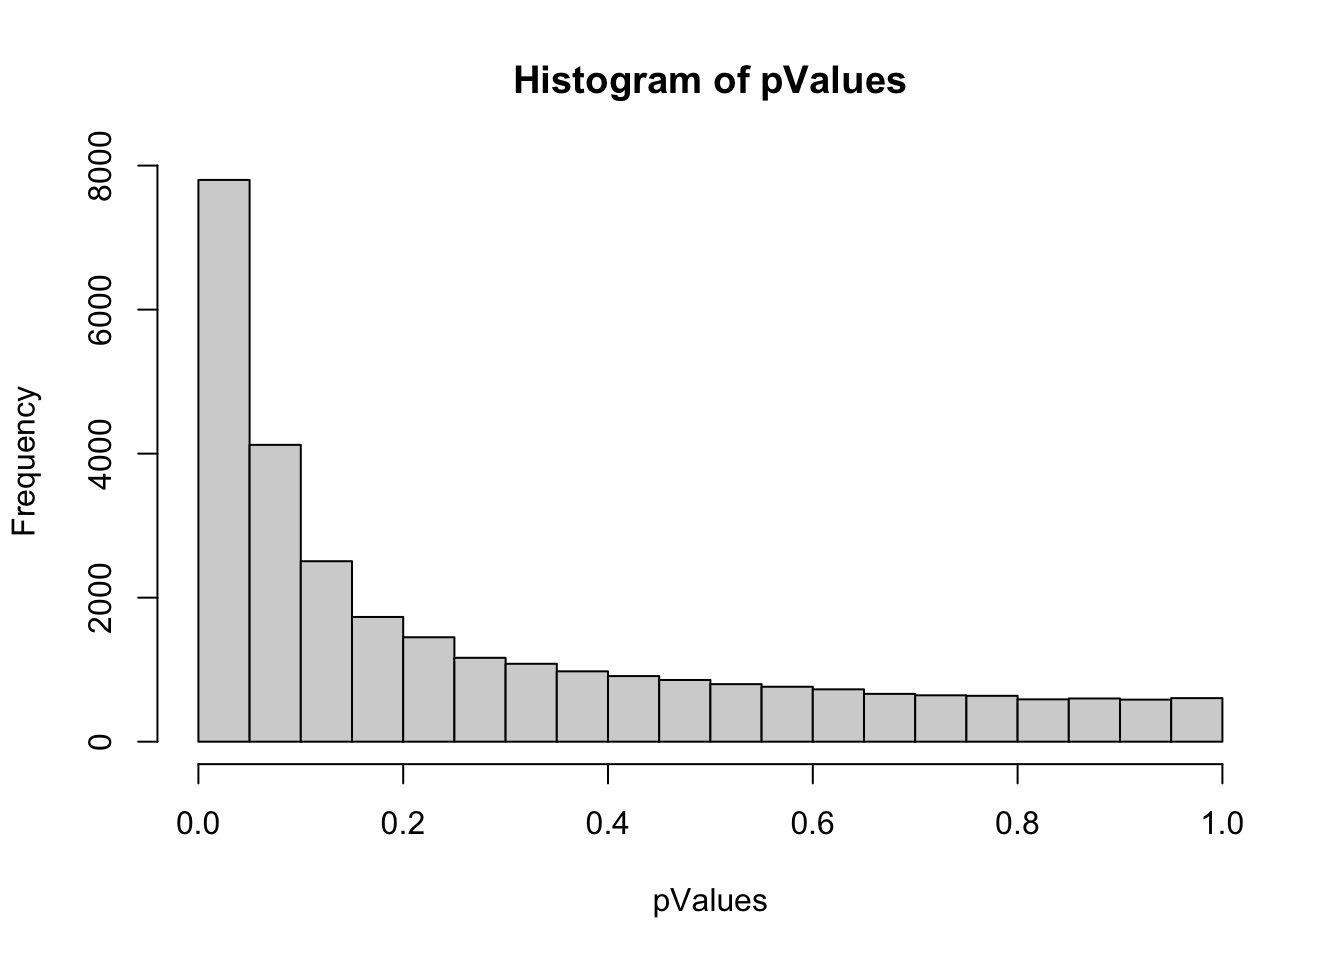
\includegraphics{TestBook_files/figure-latex/t-test-1.pdf}

Now we have a list of p-values for t-tests for each gene comparing the treated and untreated samples. Because we have run many, many tests (one for each gene), we need to adjust the p-values to correct for multiple testing. We will use an FDR correction using the ``p.adjust'' function.

\begin{Shaded}
\begin{Highlighting}[]
\CommentTok{#Adjust p-values}
\NormalTok{padj =}\StringTok{ }\KeywordTok{p.adjust}\NormalTok{(pValues, }\DataTypeTok{method=}\StringTok{"fdr"}\NormalTok{);}

\CommentTok{#Let's look at a histogram of these new values}
\KeywordTok{hist}\NormalTok{(padj);}
\end{Highlighting}
\end{Shaded}

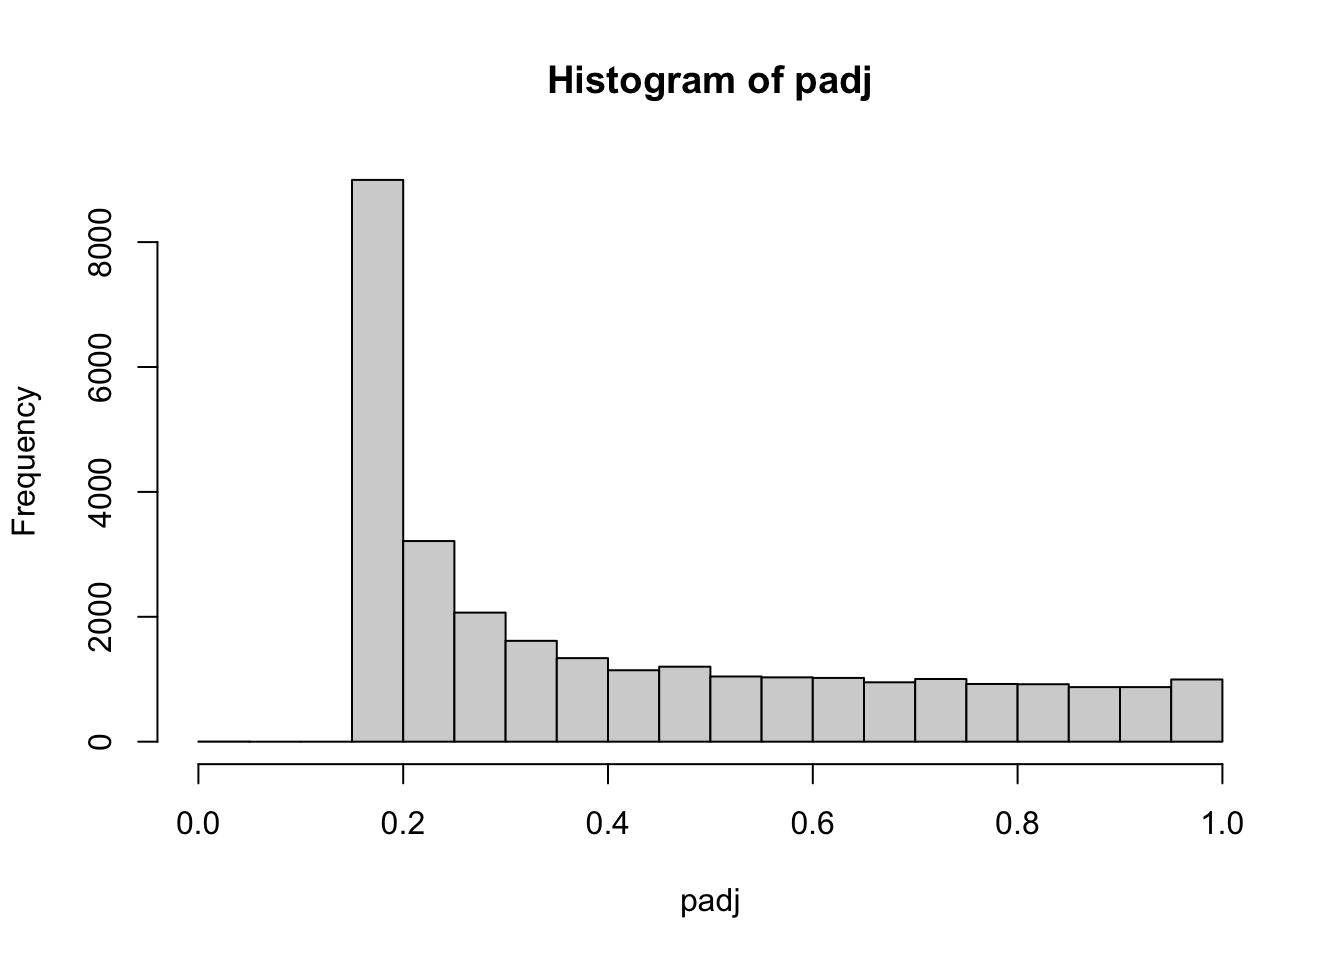
\includegraphics{TestBook_files/figure-latex/padjust-1.pdf}

\begin{Shaded}
\begin{Highlighting}[]
\CommentTok{#We can also list the smallest 10 p-values}
\CommentTok{#First we need to sort the list}
\NormalTok{padj.sorted =}\StringTok{ }\KeywordTok{sort}\NormalTok{(padj);}

\CommentTok{#Now we can view it}
\NormalTok{knitr}\OperatorTok{::}\KeywordTok{kable}\NormalTok{(}
\NormalTok{  padj[}\DecValTok{1}\OperatorTok{:}\DecValTok{10}\NormalTok{], }\DataTypeTok{caption =} \StringTok{'10 Adjusted p-values, sorted'}\NormalTok{,}
  \DataTypeTok{booktabs =} \OtherTok{TRUE}
\NormalTok{)}
\end{Highlighting}
\end{Shaded}

\begin{table}

\caption{\label{tab:padjust}10 Adjusted p-values, sorted}
\centering
\begin{tabular}[t]{lr}
\toprule
  & x\\
\midrule
10700001 & 0.1713985\\
10700002 & 0.2683722\\
10700003 & 0.1664339\\
10700004 & 0.1664339\\
10700005 & 0.1664339\\
\addlinespace
10700006 & 0.6812546\\
10700007 & 0.5660878\\
10700008 & 0.4958739\\
10700009 & 0.1915826\\
10700010 & 0.2116867\\
\bottomrule
\end{tabular}
\end{table}

After running the t-tests and adjusting them for multiple testing, we can see that we have two p-values that are still significant. These p-values belong to gene ids 10837582, 10783648. We can look up information on these genes using the tables provided on the \href{https://www.ncbi.nlm.nih.gov/geo/query/acc.cgi?acc=GPL6247}{Platform GPL6247 page}.

\hypertarget{heatmap}{%
\chapter{Heatmap}\label{heatmap}}

Heatmaps are a compact way to globally visualize large datasets. Here we will use this to view our gene expression data across all of the samples at once. We can additionally cluseter these data to try to better understand which genes (or samples) are more similar or dissimilar based on this clustering.

There are many R packages and functions to generate heatmaps. Here, we will be using the \href{https://rlbarter.github.io/superheat/}{superheat} package. To generate a basic heatmap, we simply need to pass in our dataset. We will also do some basic clustering on the data.

\begin{Shaded}
\begin{Highlighting}[]
\CommentTok{#We can use the superheat package to visualize the data}
\KeywordTok{library}\NormalTok{(superheat);}

\CommentTok{#Creates a nice heatmap}
\KeywordTok{superheat}\NormalTok{(ge.data,}
          \DataTypeTok{pretty.order.rows =}\NormalTok{ T);}
\end{Highlighting}
\end{Shaded}

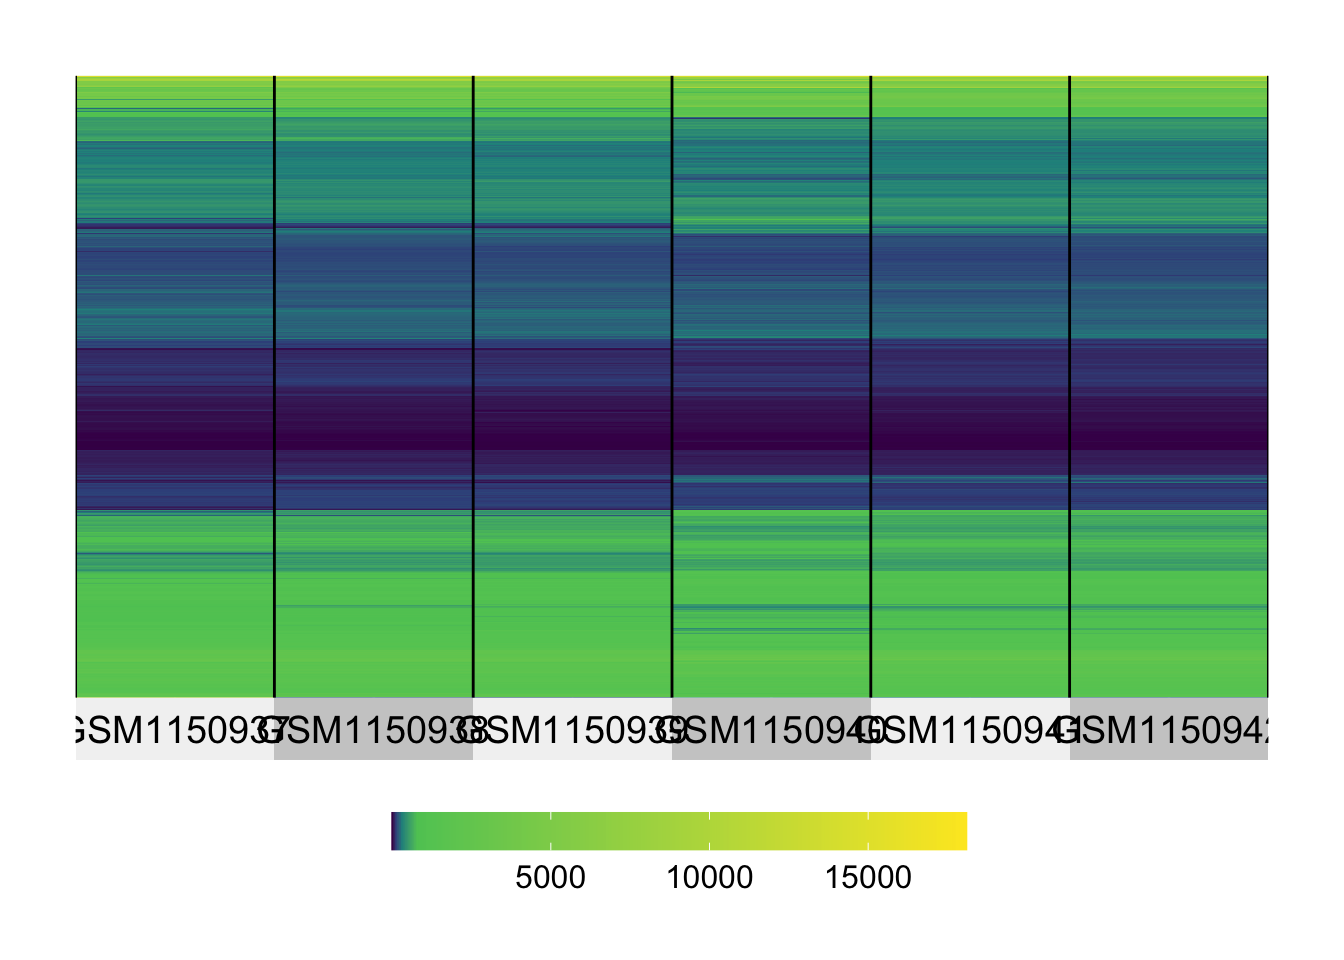
\includegraphics{TestBook_files/figure-latex/heatmap-1.pdf}

From this, we can see that there appear to be various sets of genes that cluster together. Considering we only have 6 samples and two treatment conditions, we did not cluster by samples.

\end{document}
